\documentclass{article}[jsarticle]
\usepackage[T1]{fontenc}
\usepackage[dvipdfmx]{hyperref}
\usepackage{lmodern}
\usepackage{latexsym}
\usepackage{amsfonts}
\usepackage{amssymb}
\usepackage{mathtools}
\usepackage{nccmath}
\usepackage{amsthm}
\usepackage{multirow}
\usepackage{graphicx}
\usepackage[dvipdfmx]{color}
\usepackage{wrapfig}
\usepackage{here}
\usepackage{float}
\usepackage{ascmac}
\usepackage{url}
\usepackage{listings}
\usepackage{xcolor}
\usepackage{pifont}

\lstset{
    basicstyle=\ttfamily\color{white},
    numbers=none,  % Line numbers
    numberstyle=\tiny\color{white},
    numbersep=5pt,
    tabsize=2,
    extendedchars=true,
    breaklines=true,
    keywordstyle=\color[rgb]{0.58,0.00,0.83},
    stringstyle=\color[rgb]{0.81,0.36,0.00},
    identifierstyle=\color{white},
    commentstyle=\color[rgb]{0.34,0.62,0.16},
    rulecolor=\color[rgb]{0.5,0.5,0.5},
    xleftmargin=0.1cm,    % Left margin
    xrightmargin=0.1cm,   % Right margin
    language=python,
    backgroundcolor=\color[rgb]{0.13,0.13,0.13},
    showspaces=false,
    showstringspaces=false
}



\title{機械学習 課題2}
\author{高林秀 \\ 三宅研究室 博士前期課程1年 \\ V-CampusID : 23vr008n}
\date{\today}

\begin{document}

\maketitle

\begin{abstract}
    \noindent
    本稿は本年度必修授業の機械学習の第2回レポートの答案用紙である。\par
    \noindent
    本稿は、第5回授業~第11回授業までの範囲を対象とし、各回で課された課題に対する解答を記載する。\par
    \noindent
    答案の問題番号は各章のタイトルに記載している。\par
    \noindent
    各問に対する解答は本稿に、コードなどの実行結果は別途GoogleColaboratoryのノートブックに記載した
    巻末の付録から参照できる。
\end{abstract}

\section{第5回授業 : 5/16 問題2}
    \subsection{問題文}
    次のモデルは、どのようなデータを学習する際に役に立ちそうでしょうか?
    具体的な応用先のタスク・データを想定してみてください。
    パラメータが三つある事の意味・役割も解説してください。
    またこのモデルの学習は、勾配降下法で十分でしょうか?このモデルの学習の流れを説明しなさい
    \begin{flalign*}
        & \hat{y}(x) = a_0 + a_{1}\sin x + a_2\cos x
    \end{flalign*}
    \subsection{解答}
    このモデルは、$\sin, \cos$といった周期関数が含まれているため、周期性をもつデータの学習に適していると考えられる。\par
    具体的な応用可能なタスクとして、「時刻毎の気温の変化」や「月間の株価の変動」など周期性や季節性をもつデータの学習が想定される。\par

    また各パラメータ$a_0, a_1, a_2$の役割は、モデルの式から次のように読み取ることができる。
    \begin{itemize}
        \item $a_0$ : バイアス項.モデルの予測に対して追加される定数。データの偏りによるモデルの予測値を補正する為に使用される。モデルの複雑さを抑制し過学習を予防する役割も持つ。
        \item $a_1$ : 周期関数$\sin x$に対する係数。$\sin x$の振幅を調整し、モデルに対する$\sin x$の影響度を制御する。データの周期性の大きさを調整する役割を持つ。
        \item $a_2$ : 周期関数$\cos x$に対する係数。$\cos x$の振幅を調整し、モデルに対する$\cos x$の影響度を制御する。データの周期性の大きさを調整する役割を持つ。ただし、$\sin x$の周期とは異なる位相で周期性を調整する。
    \end{itemize}
    上記3つのパラメータが独立して調整されることで、このモデルはバイアスの調整、$\sin x$と$\cos x$の周期性と影響度の調整を独立して学習することができ、よりデータに適合したモデルとすることができる。\par

    また、このモデルの学習は、勾配降下法で十分であると考えられ、その際の学習の流れは次のようになる。
    \begin{enumerate}
        \item パラメータ$a_0, a_1, a_2$を適当な値で初期化する。
        \item データ全体に対して、モデルの予測値$\hat{y}$と実際の値$y$の誤差を計算する。
        \begin{itemize}
            \item ここでは、誤差として二乗誤差:MSEなどを用いる。
        \end{itemize}
        \item 誤差関数の勾配を計算し、勾配降下法を用いてパラメータを更新する。
        \begin{itemize}
            \item 各パラメータを、その勾配に学習率をかけた値だけ引き算して更新する。
        \end{itemize}
        \item 一定の回数(エポック数)ないしは、モデルの予測値$\hat{y}$と実際の値$y$の誤差が十分小さくなるまで、2.と3.を繰り返す。
    \end{enumerate}
    この流れを前提に、このモデルの誤差関数のグラフを描画してみると、次のようになる。
    パラメータ$a_0 = 1, a_1 = 2$とし入力$x = \frac{\pi}{4}$をした場合の,$a_2$と真の値$y$との誤差:Errorをプロットしたものである。
    \begin{figure}[H]
        \centering
        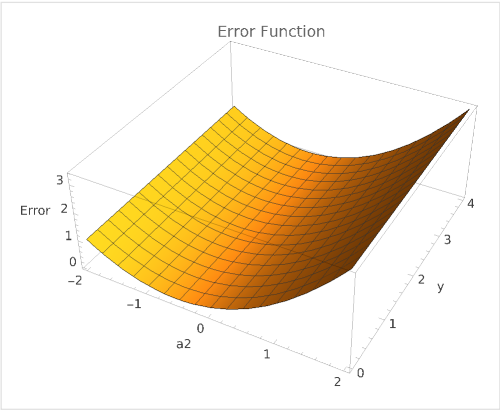
\includegraphics[scale=0.5]{./f49644b9-0517-420e-bf51-78b21e18f0ac.png}
        \caption{誤差関数のグラフ}
    \end{figure}
    このように、誤差関数は$a_2$に対して凸関数となっているため、勾配降下法によって最適解を求めることができると考えられる。


\section{第6回授業 : 問題1}

    \subsection{問題文}
    今回説明した手法を使って、重回帰の練習をしましょう。
    まず自分で何らかのデータセットを用意します(webから回帰向きのデータを検索)。
    そして、そのデータの前処理、重回帰モデルの学習、モデルの改善、ベストなモデルの選択、テスト性能の評価までを一通り行い、得られた結果について考察を加えてください。
    LASSOだけではなく、Ridgeも試してみましょう。
    モデルの学習結果から、データに関する何らかの仮説が立てられたり洞察が得られるとベストです
    \subsection{解答}
    本課題に対する解答は、以下のGoogleColabに記載している。ここでは、本課題に対して解答したソースコードのみを記載する。
    \begin{itemize}
        \item ファイル(code.ipynb) : \url{https://colab.research.google.com/drive/1Zx4wYZWsR5Ge_Phy0yRFJbOT9IO5puMr?usp=sharing}
        \item 使用データセット(SSDSE-C-2023.csv) : \url{https://drive.google.com/file/d/1-LLPqbwy09z1qwkAQnVIXE2dTMomZiyc/view?usp=drive_link}
    \end{itemize}


\section{第7回授業 : 問題1}

    \subsection{問題文}
    クロスエントロピーの勾配と決定境界について、以下の問に答えよ。
    \begin{enumerate}
        \item $a$に関する勾配の導出を(丁寧に)まとめよ(写経)。
        \item $b$に関する勾配も丁寧に導出せよ。
        \item 決定境界を直線ではなく、放物線のように曲げるにはロジスティック回帰の式をどう変更すればいいか?
        \begin{itemize}
            \item 言葉でふんわり説明ではなく、数式をきちんと使って「アルゴリズム」にできるような議論を。
        \end{itemize}
    \end{enumerate}
    \subsection{解答}

\section{第10回授業 : 6/20 問題1}

    \subsection{問題文}
    多クラス分類と、識別関数の図形的な仕組みについて、以下の問に答えよ。
    \begin{enumerate}
        \item p.18の絵において、$f_k = \text{一定値}$の直線はどの様に図示されるか?傾きは適当で良いが、$k = 0,1,2$に対して(共通の一定値に対して)図示せよ。
        \item この図の半直線$f_0 = f_1$に沿ったまま無限遠方へ移動したとする。この時3つのクラスに対する確率の値は幾つになるか?
        \begin{itemize}
            \item 真面目に計算して証明する必要はない。簡単な理由があればいい。
        \end{itemize}
    \end{enumerate}
    \subsection{解答}

\section{第11回授業 : 6/27 問題1}

    \subsection{問題文}
    二次計画問題と有効な制約について、以下の問に答えよ。
    \begin{enumerate}
        \item p.51の問題を解きなさい。
        \item p.60 ~ p.63で得られた双対問題を解いて、\ding{172}と同じ解が求まることえお確認しなさい。
    \end{enumerate}
    \subsection{解答}

    

\end{document}